% CHKTEX-FILE 1
\documentclass[letterpaper,10.5pt]{article}
\usepackage[utf8]{inputenc}
\usepackage[T1]{fontenc}
\usepackage[english,spanish,mexico,es-lcroman]{babel}
% Standard packages
\usepackage{float}
\usepackage{ifthen}
\usepackage{xspace}
\usepackage{amsmath}
\usepackage{xstring}
\usepackage{wrapfig}
\usepackage{booktabs}
\usepackage{csquotes}
\usepackage{fancyhdr}
\usepackage{fancyvrb}
\usepackage{geometry}
\usepackage{graphicx}
\usepackage{lastpage}
\usepackage{listings}
\usepackage{multicol}
\usepackage{multirow}
\usepackage{tabularx}
\usepackage{algorithm}
\usepackage{textgreek}
\usepackage[justification=centering]{subcaption}
\usepackage{algpseudocode}
\usepackage[all]{nowidow}
\usepackage[inline]{enumitem}
\usepackage[usenames,dvipsnames]{xcolor}
% Packages to be loaded later
\usepackage{tikz}
\usepackage{cancel}
\usepackage{tcolorbox}
% Include fullpage images with \includepdf
% \usepackage{pdfpages}
% Referencing
\usepackage{varioref}
\usepackage{hyperref}
\usepackage[noabbrev,nameinlink,spanish]{cleveref}
\usepackage[square, comma, numbers, sort&compress]{natbib}


\newcommand{\lpar}{(}\newcommand{\rpar}{)} %CHKTEX 9
\newcommand{\IIC}{I\textsuperscript{2}C\xspace}
\newcommand{\GND}{\textsc{Gnd}\xspace}
\newcommand{\VCC}{\textsc{Vcc}\xspace}
\newcommand{\VDD}{\textsc{Vdd}\xspace}
\newcommand{\textbi}[1]{\textbf{\textit{#1}}}
\newcommand{\degreesC}[1]{%
	#1\textsuperscript{o}C\xspace{}%
}
\newcommand{\degreesF}[1]{%
	#1\textsuperscript{o}F\xspace{}%
}

% \newcommand{\VCC}{V\textsubscript{CC}\xspace{}}
% \newcommand{\GND}{\textsc{Gnd}\xspace{}}
% CHKTEX-FILE 26
% CHKTEX-FILE 36

\tcbuselibrary{most}
% \tcbuselibrary{listings,breakable}
% \usetikzlibrary{shadings,shadows}
% \usetikzlibrary{decorations.pathmorphing}
% \usetikzlibrary{patterns}
% \usetikzlibrary{spy}
% \usetikzlibrary{arrows.meta}

\newtcolorbox{importantbox}[1]{%
	enhanced,
	colback=red!5!white,%
	colframe=red!75!black,%
	fonttitle=\bfseries,%
	center title,
	title={#1},%
	drop fuzzy shadow
}

\newtcolorbox{marker}[1][]{%
	enhanced,
	before skip=2mm,after skip=3mm,
	boxrule=0.4pt,left=5mm,right=2mm,top=1mm,bottom=1mm,
	colback=yellow!50,
	colframe=yellow!20!black,
	sharp corners,rounded corners=southeast,arc is angular,arc=3mm,
%	underlay={%
%		\path[fill=tcbcolback!80!black] ([yshift=3mm]interior.south east)--++(-0.4,-0.1)--++(0.1,-0.2);
%		\path[draw=tcbcolframe,shorten <=-0.05mm,shorten >=-0.05mm] ([yshift=3mm]interior.south east)--++(-0.4,-0.1)--++(0.1,-0.2);
%		\path[fill=yellow!50!black,draw=none] (interior.south west) rectangle node[white]{\Huge\bfseries !} ([xshift=4mm]interior.north west);
%	},
	drop fuzzy shadow,#1
}

%CHKTEX-FILE 1
%CHKTEX-FILE 7
%CHKTEX-FILE 9
% Default fixed font does not support bold face
\DeclareFixedFont{\ttb}{T1}{txtt}{bx}{n}{8} % for bold
\DeclareFixedFont{\ttm}{T1}{txtt}{m}{n}{8}  % for normal

% Custom colors
\usepackage{color}
\definecolor{keywordsColor}{rgb}{0,0,0.5}
\definecolor{customColor}{rgb}{0.6,0,0}
\definecolor{stringColor}{rgb}{0,0.5,0}

% Code highlighting python
\renewcommand{\ttdefault}{pcr}
\lstset{
	language=Python,                              % the language of the code (can be overrided per snippet)
	backgroundcolor=\color{white},                % choose the background color
	basicstyle=\footnotesize\ttfamily,            % the size of the fonts that are used for the code
	breakatwhitespace=false,                      % sets if automatic breaks should only happen at whitespace
	breaklines=true,                              % sets automatic line breaking
	captionpos=t,                                 % sets the caption-position to bottom
	commentstyle=\color{gray},                    % comment style
	deletekeywords={},                            % if you want to delete keywords from the given language
%	escapeinside={\%*}{*)},                       % if you want to add LaTeX within your code
	extendedchars=true,                           % lets you use non-ASCII characters; for 8-bits encodings only, does not work with UTF-8
	frame=tb,                                     % adds a frame around the code
	keepspaces=true,                              % keeps spaces in text, useful for keeping indentation of code (possibly needs columns=flexible)
	keywordstyle=\color{keywordsColor}\bfseries,  % keyword style
	numbers=left,                                 % where to put the line-numbers; possible values are (none, left, right)
	numbersep=5pt,                                % how far the line-numbers are from the code
	numberstyle=\tiny\color{gray},                % the style that is used for the line-numbers
	rulecolor=\color{black},                      % if not set, the frame-color may be changed on line-breaks within not-black text (e.g. comments (green here))
	showspaces=false,                             % show spaces everywhere adding particular underscores; it overrides 'showstringspaces'
	showstringspaces=false,                       % underline spaces within strings only
	showtabs=false,                               % show tabs within strings adding particular underscores
	stepnumber=1,                                 % the step between two line-numbers. If it's 1, each line will be numbered
	stringstyle=\color{stringColor},              % string literal style
	tabsize=2,                                    % sets default tabsize to 2 spaces
	title=\lstname,                               % show the filename of files included with \lstinputlisting; also try caption instead of title
	columns=fixed,                                % Using fixed column width (for e.g. nice alignment)
	otherkeywords={self},                         % if you want to add more keywords to the set
	emphstyle=\color{customColor}\bfseries,       % Custom highlighting style
	emph={__init__,__main__,True,False,None},     % Custom highlighting keywords
	xleftmargin=1cm,                              % Left margin
	xrightmargin=1cm,                             % Right margin
	% Unicode compatibility
	inputencoding=utf8,
	literate={%
	            {Á}{{\'a}}1 {É}{{\'E}}1 {Í}{{\'I}}1 {Ó}{{\'O}}1 {Ú}{{\'U}}1%
	            {á}{{\'a}}1 {é}{{\'e}}1 {í}{{\'i}}1 {ó}{{\'o}}1 {ú}{{\'u}}1%
	            {À}{{\`A}}1 {È}{{\'E}}1 {Ì}{{\`I}}1 {Ò}{{\`O}}1 {Ù}{{\`U}}1%
	            {à}{{\`a}}1 {è}{{\`e}}1 {ì}{{\`i}}1 {ò}{{\`o}}1 {ù}{{\`u}}1%
	            {Ä}{{\"A}}1 {Ë}{{\"E}}1 {Ï}{{\"I}}1 {Ö}{{\"O}}1 {Ü}{{\"U}}1%
	            {ä}{{\"a}}1 {ë}{{\"e}}1 {ï}{{\"i}}1 {ö}{{\"o}}1 {ü}{{\"u}}1%
	            {Â}{{\^A}}1 {Ê}{{\^E}}1 {Î}{{\^I}}1 {Ô}{{\^O}}1 {Û}{{\^U}}1%
	            {â}{{\^a}}1 {ê}{{\^e}}1 {î}{{\^i}}1 {ô}{{\^o}}1 {û}{{\^u}}1% CHKTEX 19
	            {Ã}{{\~a}}1 {Ẽ}{{\~E}}1 {Ĩ}{{\~I}}1 {Õ}{{\~O}}1 {Ũ}{{\~U}}1 {Ñ}{{\~N}}1%
	            {ã}{{\~a}}1 {ẽ}{{\~e}}1 {ĩ}{{\~i}}1 {õ}{{\~o}}1 {ũ}{{\~u}}1 {ñ}{{\~n}}1%
	            {œ}{{\oe}}1 {Œ}{{\OE}}1 {æ}{{\ae}}1 {Æ}{{\AE}}1 {ß}{{\ss}}1%
	            {ç}{{\c c}}1 {Ç}{{\c C}}1 {ø}{{\o}}1 {å}{{\r a}}1 {Å}{{\r A}}1%
	            {€}{{\EUR}}1 {£}{{\pounds}}1 {×}{{\(\times\)}}1% CHKTEX 21
	            {°}{{\textsuperscript{o}}}1%
	            {¹}{{\textsuperscript{1}}}1%
	            {²}{{\textsuperscript{2}}}1%
	            {³}{{\textsuperscript{3}}}1%
	            {⁴}{{\textsuperscript{4}}}1% CHKTEX 19
	            {⁵}{{\textsuperscript{5}}}1% CHKTEX 19
	            {⁶}{{\textsuperscript{6}}}1% CHKTEX 19
	            {⁷}{{\textsuperscript{7}}}1% CHKTEX 19
	            {⁸}{{\textsuperscript{8}}}1% CHKTEX 19
	            {⁹}{{\textsuperscript{9}}}1% CHKTEX 19
	            {⁰}{{\textsuperscript{0}}}1% CHKTEX 19
%	            {A}{{\textAlpha}}1
	            {α}{{\textalpha}}1%
%	            {B}{{\textBeta}}1
	            {β}{{\textbeta}}1%
	            {Γ}{{\textGamma}}1
	            {γ}{{\textgamma}}1%
	            {Δ}{{\textDelta}}1
	            {δ}{{\textdelta}}1% CHKTEX 19
%	            {E}{{\textEpsilon}}1
	            {ϵ}{{\textepsilon}}1%
%	            {Z}{{\textZeta}}1
	            {ζ}{{\textzeta}}1%
%	            {H}{{\textEta}}1
	            {η}{{\texteta}}1%
	            {Θ}{{\textTheta}}1
	            {θ}{{\texttheta}}1%
%	            {I}{{\textIota}}1
	            {ι}{{\textiota}}1%
%	            {K}{{\textKappa}}1
	            {κ}{{\textkappa}}1%
	            {Λ}{{\textLambda}}1
	            {λ}{{\textlambda}}1%
%	            {M}{{\textMu}}1
	            {μ}{{\textmu}}1%
%	            {N}{{\textNu}}1
	            {ν}{{\textnu}}1%
	            {Ξ}{{\textXi}}1
	            {ξ}{{\textxi}}1%
%	            {O}{{\textOmikron}}1
%	            {o}{{\textomikron}}1%
	            {Π}{{\textPi}}1
	            {π}{{\textpi}}1%
%	            {P}{{\textRho}}1
	            {ρ}{{\textrho}}1%
	            {Σ}{{\textSigma}}1
	            {σ}{{\textsigma}}1%
%	            {T}{{\textTau}}1
	            {τ}{{\texttau}}1%
	            {ϒ}{{\textUpsilon}}1
	            {υ}{{\textupsilon}}1%
	            {Φ}{{\textPhi}}1
	            {ϕ}{{\textphi}}1%
%	            {X}{{\textChi}}1
	            {χ}{{\textchi}}1%
	            {Ψ}{{\textPsi}}1
	            {ψ}{{\textpsi}}1%
	            {Ω}{{\textOmega}}1
	            {ω}{{\textomega}}1%
	            {ζ}{{\varsigma}}1%
%	            {}{{\straightphi}}1%
%	            {}{{\scripttheta}}1%
%	            {}{{\straighttheta}}1%
%	            {}{{\straightepsilon}}1%
	         },
}

\lstdefinestyle{c_with_comments}%
{
	language     = c,
	morecomment  = [l]{//},
	morecomment  = [s]{/*}{*/},
	breaklines,
}

\lstdefinestyle{c_without_comments}%
{
	style        = c_with_comments,
	% numbers      = none,
	% keepspaces   = false,
	morecomment  = [l][\nullfont]{//},
	morecomment  = [is]{//}{\^^M},
	morecomment  = [is]{/*}{*/},
}

\lstdefinelanguage{conf}
{
	basicstyle=\ttfamily\small,
	columns=fullflexible,
	morecomment=[s][\color{Orchid}\bfseries]{[}{]},
	morecomment=[l]{\#},
	morecomment=[l]{;},
	commentstyle=\color{gray}\ttfamily,
	% morekeywords={},
	% otherkeywords={=,:},
	% keywordstyle={\color{Green}\bfseries}
}

% \captionsetup[lstlisting]{font={small,tt}}
\captionsetup[lstlisting]{%
	font={small},
}



\DefineVerbatimEnvironment{Verbatim}{Verbatim}{%
	fontsize=\footnotesize,%
	frame=leftline,%
	framesep=2em,    % separation between frame and text
}

\RecustomVerbatimCommand{\VerbatimInput}{VerbatimInput}{%
	fontsize=\footnotesize,
%	frame=lines,            % top and bottom rule only
	frame=leftline,         % left rule only
	numbers=left,           % Line numbers on the left
	numbersep=0.25em,       % Gap between numbers and verbatim lines
	xleftmargin=4em,        % Indentation to add at the start of each line
	xrightmargin=4em,       % Right margin to add after each line
	framesep=0.5em,         % separation between frame and text
	rulecolor=\color{Gray}, % Color of the lines
	labelposition=topline,  %
	samepage=false,         % When true, prevents verbatim environment from
	                        % being broken between pages
%	commandchars=\|\(\),    % escape character and argument delimiters for
	                        % commands within the verbatim
%	commentchar=*           % comment character
}


\hypersetup{
	hidelinks,
	colorlinks=true,
	linkcolor=Blue,
	filecolor=OliveGreen,
	urlcolor=RoyalPurple,
	pdfauthor={Mauricio Matamoros},
%	pdftitle={Práctica 0X – Fundamentos de Sistemas Embebidos},
% 	pdfsubject={The Subject},
% 	pdfkeywords={Some Keywords},
% 	pdfproducer={Latex with hyperref, or other system},
% 	pdfcreator={pdflatex, or other tool}
}

\captionsetup{%
	font=small
}

\geometry{%
	margin=2cm,
	% top=3cm,
	bottom=3cm,
	% left=2cm,
	% right=2cm,
	% inner=2cm,
	% outer=2cm,
	% headheight=,
	% footsep=,
	% footskip=,
}

\pagestyle{fancy}
\renewcommand{\headrulewidth}{0.0pt}
\lhead{}
\chead{}
\rhead{}
\lfoot{}
\cfoot{}
\rfoot{Página~\thepage~de~\pageref{LastPage}}

\crefname{table}{tabla}{tablas}
\Crefname{table}{Tabla}{Tablas}
\crefname{section}{sección}{secciones}
\Crefname{section}{Sección}{Secciones}
\crefname{subsection}{subsección}{subsecciones}
\Crefname{subsection}{Subsección}{Subsecciones}
\crefname{listing}{código de ejemplo}{códigos de ejemplo}
\Crefname{listing}{Código de Ejemplo}{Códigos de Ejemplo}
\renewcommand*{\lstlistingname}{Código ejemplo}


\author{\footnotesize Autor: José Mauricio Matamoros de Maria y Campos}
\title{Práctica 2:\\Instalación de Windows 10 IoT Core en la Raspberry Pi\\
{\large Fundamentos de Sistemas Embebidos}}
\date{}

% Document body
\begin{document}
\maketitle

\section{Objetivo}%
\label{sec:objective}
El alumno aprenderá a instalar un sistema operativo basado en Windows, como sistema operativo embebido, en una tarjeta microcontroladora.

% \section{Introducción}%
% \label{sec:introduction}
% Raspbian es el sistema operativo más popular para Raspberry Pi, además de ser el único con soporte oficial.
% Raspbian es una distribución de Linux basada en Debian, optimizado para la Raspberry Pi y que permite a esta operar como una PC.~La distro incorpora terminal y navegador web entre otros programas.

\section{Instrucciones}%
\label{sec:instructions}

Para Windows 10 en la Raspberry se necesita lo siguiente:
\begin{itemize}[nosep]
	\item Una computadora cono Microsoft Windows 10 capaz de leer y escribir tarjetas microSD (o bien un adaptador para la misma) y conexión a internet para descargar la imagen de Windows 10 IoT Core.
	\item Una tarjeta de memoria microSD de al menos 16 GB (se recomiendan 32GB)
	\item Una Raspberry Pi 2 o posterior (se requieren versiones con 1GB de ram o más)
	\item Un monitor con soporte para HDMI
	\item Un teclado USB
	\item Un mouse USB
	\item Una fuente de alimentación de 5V@1A con adaptador microUSB
\end{itemize}

\paragraph*{IMPORTANTE:} Se necesita Windows 10 para poder instalar Windows 10 IoT Core en una Raspberry Pi. Si no cuenta con una máquina que tenga Windows 10 precargado, no podrá realizarse esta práctica. Debido a que Windows 10 es software propietario, la realización de esta práctica no es obligatoria.

% %% %%%%%%%%%%%%%%%%%%%%%%%%%%%%%%%%%%%%%%%%%%%%%%%%%%%%%%%%%%%%%%%%%%
%
% Step 1
%
% %% %%%%%%%%%%%%%%%%%%%%%%%%%%%%%%%%%%%%%%%%%%%%%%%%%%%%%%%%%%%%%%%%%%
\subsection{Paso 1: Descargar Windows 10 IoT Core}%
\label{sec:step1}

\begin{enumerate}
	\item Vaya a centro de desarrollo de Windows 10 (Windows 10 developer center).
	\item De clic en \textit{Get Windows 10 IoT Core Dashboard} para descargar la aplicación requerida.
	\begin{figure}[H]
		\centering%
		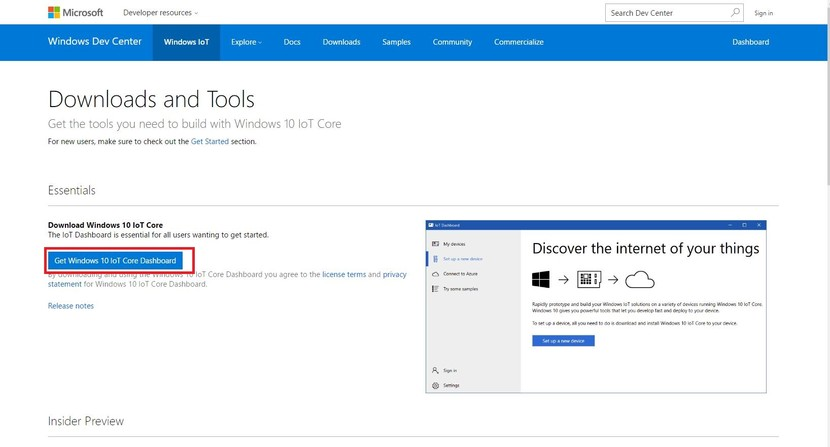
\includegraphics[width=0.5\columnwidth,height=8cm,keepaspectratio]{img/p02-01.jpg} %CHKTEX 8
		\caption{Descarga de Windows 10 IoT Core Dashboard}
		\label{fig:dashboard-download} %CHKTEX 24
	\end{figure}
	También puede utilizarse ésta liga:
	\url{https://docs.microsoft.com/en-us/windows/iot-core/downloads}

	\item Instale la aplicación y ejecútela.

	\item Seleccione la opción \textit{configurar un nuevo dispositivo} (Set up a new device) en la barra lateral y seleccione configurar Windows 10 IoT Core en una Raspberry Pi tal como se muestra en la \Cref{fig:setup-new-device}
	Tenga cuidado de seleccionar la letra de unidad correcta de la memoria microSD, una conexión a internet, y de anorar un nombre de dispositivo y contraseña.
    \begin{figure}
		\centering%
		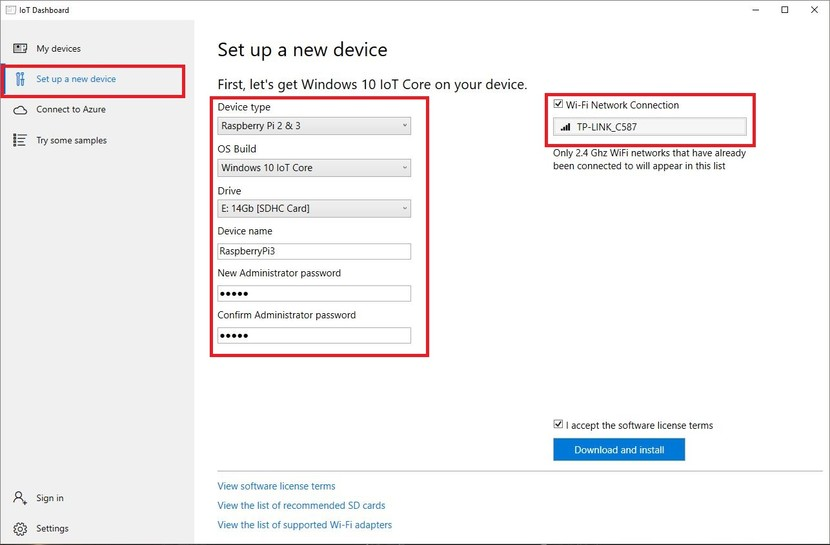
\includegraphics[width=0.9\columnwidth,height=8cm,keepaspectratio]{img/p02-02.jpg} %CHKTEX 8
		\caption{Configuración de la descarga de Windows 10 IoT Core}
		\label{fig:setup-new-device} %CHKTEX 24
	\end{figure}

	\item De clic en el botón \textit{Descargar e instalar} (Download and install).

\end{enumerate}

La aplicación descargará los archivos requeridos de los servidores Microsoft y los exscribirá en la memoria microSD. % CHKTEX 13
Tenga en cuenta que este proceso puede llevar varias horas, especialmente con conexiones lentas.

Windows 10 IoT Core Dashboard le notificará cuando el proceso de descarga y copiado de datos haya concluído (véase \Cref{fig:image-installed}).

\begin{figure}
	\centering%
	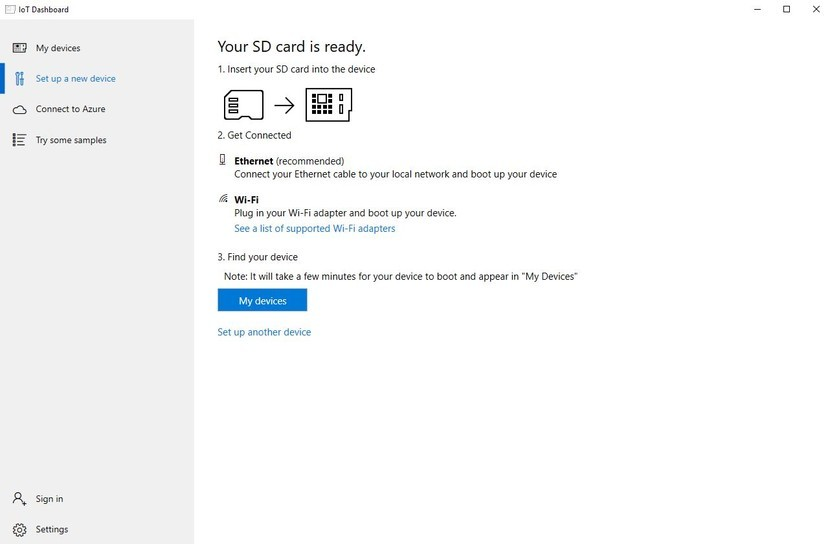
\includegraphics[width=0.9\columnwidth,height=8cm,keepaspectratio]{img/p02-03.jpg} %CHKTEX 8
	\caption{Imagen de Windows 10 IoT Core instalada en la memoria microSD}
	\label{fig:image-installed} %CHKTEX 24
\end{figure}

% %% %%%%%%%%%%%%%%%%%%%%%%%%%%%%%%%%%%%%%%%%%%%%%%%%%%%%%%%%%%%%%%%%%%
%
% Step 2
%
% %% %%%%%%%%%%%%%%%%%%%%%%%%%%%%%%%%%%%%%%%%%%%%%%%%%%%%%%%%%%%%%%%%%%
\subsection{Paso 2: Configuración de Windows 10 IoT Core en la Raspberry Pi}%
\label{sec:step2}

Una vez terminados la descarga y copiado de datos en la microSD, inserte la tarjeta en la Raspberry Pi.
A continuación, conecte la Raspberry Pi a un monitor usando el puerto HDMI, así como a un teclado y ratón.
Finalmente, conecte la Raspberry Pi a la alimentación.

La raspberry Pi tardará aproximadamente dos minutos en arrancar y mostrará una pantalla de carga durante el proceso de arranque (véase \Cref{fig:boot}).

\begin{figure}[H]
	\centering%
	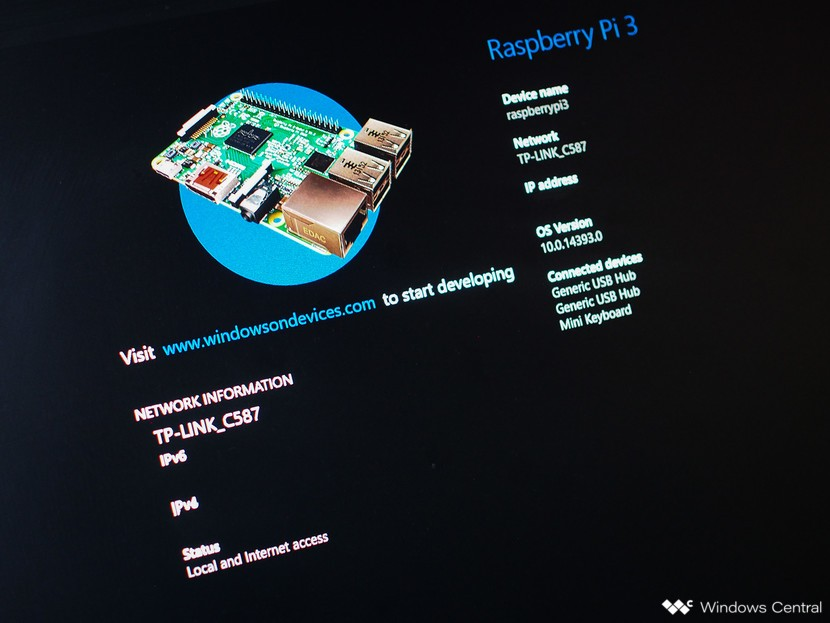
\includegraphics[width=0.9\columnwidth,height=8cm,keepaspectratio]{img/p02-04.jpg} %CHKTEX 8
	\caption{Arranque de Windows 10 IoT Core en la Raspberry Pi}
	\label{fig:boot} %CHKTEX 24
\end{figure}

Notará que a diferencia de otros sistemas Windows, hay muy poco que configurar a la Raspberry Pi.
Se le solicitará que elija el idioma y que entre la contraseña de la red inalámbrica con la que desea conectarse a la Internet (si su Raspberry Pi está equipada con WiFi).

Notará que el ambiente es bastante austero y carece de aplicaciones.
Esto es debido a que una vez que se instale una aplicación en la Raspberry Pi, Windows desaparecerá y sólo le permitirá interactuar con la App.

Si la Raspberry Pi está conectada a la red local, podrá ver que ésta aparece en la aplicación de desarrollo (\Cref{fig:listed-pi}).

\begin{figure}[H]
	\centering%
	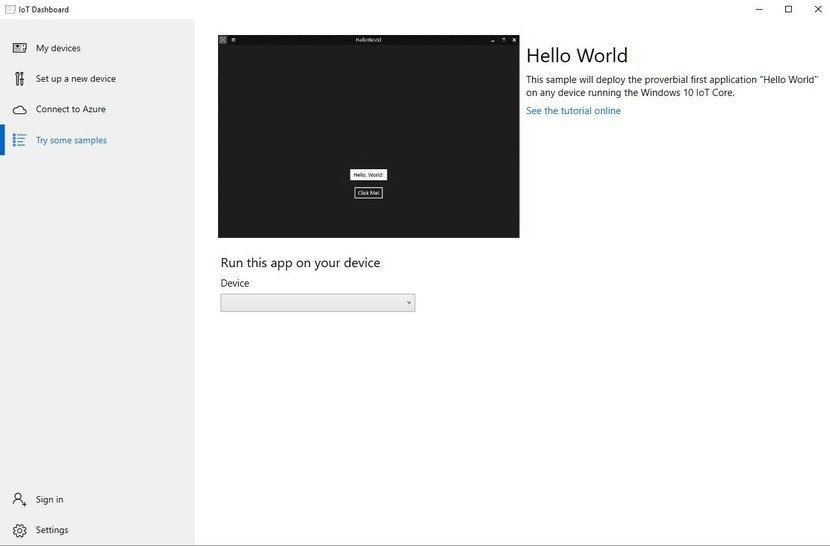
\includegraphics[width=0.9\columnwidth,height=8cm,keepaspectratio]{img/p02-05.jpg} %CHKTEX 8
	\caption{Raspberry Pi en la Windows 10 IoT Core Dashboard}
	\label{fig:listed-pi} %CHKTEX 24
\end{figure}


\end{document}
